% Options for packages loaded elsewhere
\PassOptionsToPackage{unicode}{hyperref}
\PassOptionsToPackage{hyphens}{url}
\documentclass[
]{article}
\usepackage{xcolor}
\usepackage{amsmath,amssymb}
\setcounter{secnumdepth}{-\maxdimen} % remove section numbering
\usepackage{iftex}
\ifPDFTeX
  \usepackage[T1]{fontenc}
  \usepackage[utf8]{inputenc}
  \usepackage{textcomp} % provide euro and other symbols
\else % if luatex or xetex
  \usepackage{unicode-math} % this also loads fontspec
  \defaultfontfeatures{Scale=MatchLowercase}
  \defaultfontfeatures[\rmfamily]{Ligatures=TeX,Scale=1}
\fi
\usepackage{lmodern}
\ifPDFTeX\else
  % xetex/luatex font selection
\fi
% Use upquote if available, for straight quotes in verbatim environments
\IfFileExists{upquote.sty}{\usepackage{upquote}}{}
\IfFileExists{microtype.sty}{% use microtype if available
  \usepackage[]{microtype}
  \UseMicrotypeSet[protrusion]{basicmath} % disable protrusion for tt fonts
}{}
\makeatletter
\@ifundefined{KOMAClassName}{% if non-KOMA class
  \IfFileExists{parskip.sty}{%
    \usepackage{parskip}
  }{% else
    \setlength{\parindent}{0pt}
    \setlength{\parskip}{6pt plus 2pt minus 1pt}}
}{% if KOMA class
  \KOMAoptions{parskip=half}}
\makeatother
\usepackage{longtable,booktabs,array}
\newcounter{none} % for unnumbered tables
\usepackage{calc} % for calculating minipage widths
% Correct order of tables after \paragraph or \subparagraph
\usepackage{etoolbox}
\makeatletter
\patchcmd\longtable{\par}{\if@noskipsec\mbox{}\fi\par}{}{}
\makeatother
% Allow footnotes in longtable head/foot
\IfFileExists{footnotehyper.sty}{\usepackage{footnotehyper}}{\usepackage{footnote}}
\makesavenoteenv{longtable}
\usepackage{graphicx}
\makeatletter
\newsavebox\pandoc@box
\newcommand*\pandocbounded[1]{% scales image to fit in text height/width
  \sbox\pandoc@box{#1}%
  \Gscale@div\@tempa{\textheight}{\dimexpr\ht\pandoc@box+\dp\pandoc@box\relax}%
  \Gscale@div\@tempb{\linewidth}{\wd\pandoc@box}%
  \ifdim\@tempb\p@<\@tempa\p@\let\@tempa\@tempb\fi% select the smaller of both
  \ifdim\@tempa\p@<\p@\scalebox{\@tempa}{\usebox\pandoc@box}%
  \else\usebox{\pandoc@box}%
  \fi%
}
% Set default figure placement to htbp
\def\fps@figure{htbp}
\makeatother
\setlength{\emergencystretch}{3em} % prevent overfull lines
\providecommand{\tightlist}{%
  \setlength{\itemsep}{0pt}\setlength{\parskip}{0pt}}
\usepackage{bookmark}
\IfFileExists{xurl.sty}{\usepackage{xurl}}{} % add URL line breaks if available
\urlstyle{same}
\hypersetup{
  hidelinks,
  pdfcreator={LaTeX via pandoc}}

\author{}
\date{}

\begin{document}

\section{\texorpdfstring{IRC-Bench: Recognizing Entities from Contextual
Cues\\
in First-Person
Reminiscences}{IRC-Bench: Recognizing Entities from Contextual Cues in First-Person Reminiscences}}\label{irc-bench-recognizing-entities-from-contextual-cues-in-first-person-reminiscences}

Alexander Apartsin\textsuperscript{1} ~~ Eden Moran\textsuperscript{2}
~~ Yehudit Aperstein\textsuperscript{2}

\textsuperscript{1}School of Computer Science, HIT-Holon Institute of
Technology, Holon, Israel\\
\textsuperscript{2}Intelligent Systems, Afeka Academic College of
Engineering, Tel Aviv, Israel

\subsection{Abstract}\label{abstract}

People sharing personal reminiscences routinely reference entities
through contextual cues alone, without explicit naming. We extend
implicit entity recognition from short social-media text to long-form
reminiscence narratives, where entity cues are distributed across
multiple clauses. We release \emph{IRC-Bench}, a benchmark of 25,136
samples derived from 12,337 Wikidata-linked entities across 1,994 oral
history transcripts spanning 11 thematic domains. We formalize the
\emph{non-locality} property of implicit references: recognition cues
are distributed across non-contiguous clauses, distinguishing this task
from NER, entity linking, and coreference resolution. We evaluate 19
configurations spanning open-world LLM generation, closed-world dense
retrieval, hybrid RAG, and fine-tuning. QLoRA-adapted Llama 3.1 8B
achieves 38.94\% exact match (51.59\% Jaccard), while fine-tuned DPR
reaches 35.38\% Hit@1 and 71.49\% Hit@10. Chain-of-thought prompting
consistently degrades performance, and RAG underperforms direct LLM
inference. All data, code, and evaluation tools are publicly released.

\subsection{1 ~ Introduction}\label{introduction}

Reminiscence, the act of recalling and sharing personal memories, plays
a central role in human social life. In clinical settings, reminiscence
therapy reduces depression in older adults {[}1{]}, while in archival
contexts, recorded reminiscences preserve cultural knowledge {[}2{]}. A
defining characteristic of reminiscence narratives is that speakers
reference people, places, and events through contextual cues rather than
explicit naming, trusting the listener to fill in the gaps. This
implicit referencing creates a fundamental challenge for automated
systems that seek to index, search, or analyze these narratives.

Consider the following passage from a Japanese American reminiscence:

Entity-Grounded Narrative (EGN)

"The attack on Pearl Harbor was the event that changed everything for
Japanese Americans like me. After December 7, 1941, suspicion and hatred
grew, and we were treated as enemy aliens despite being American
citizens. It was because of Pearl Harbor that the government issued
Executive Order 9066 and started the forced relocation."

Entity-Elided Narrative (EEN)

"The surprise attack on a naval base in Hawaii was the event that
changed everything for Japanese Americans like me. After December 7,
1941, suspicion and hatred grew, and we were treated as enemy aliens
despite being American citizens. It was because of that attack that the
government issued an order and started the forced relocation."

\textbf{Gold entity:} Attack on Pearl Harbor (Q52418) ~\textbar~
\textbf{Cues:} December 7, 1941; naval base in Hawaii; Executive Order
9066; forced relocation

A human reader identifies the Attack on Pearl Harbor from the
constellation of cues: the date, the Hawaiian naval base, the executive
order, the internment. No single phrase names the entity; recognition
depends on integrating knowledge distributed across the entire passage.
This phenomenon falls between existing NLP tasks. Named Entity
Recognition (NER) identifies explicit spans {[}3, 4{]}. Entity Linking
(EL) resolves those spans to knowledge base entries {[}5, 6{]}.
Coreference resolution requires at least one explicit mention as
antecedent {[}7{]}. In implicit entity references, the entity is never
named; there is no span to extract, no mention to link, no antecedent to
resolve.

Our contributions are: (1) We extend implicit entity recognition from
tweets {[}8, 9{]} to long-form reminiscence narratives and formalize the
\emph{non-locality property} of implicit references. (2) We release
IRC-Bench, a benchmark of 25,136 samples from 12,337 Wikidata-linked
entities across 1,994 transcripts, with entity-level train/dev/test
splits ensuring zero entity overlap. (3) We systematically compare 19
configurations spanning four paradigms (generative LLM, dense retrieval,
RAG, fine-tuning), revealing that fine-tuning doubles performance,
chain-of-thought reasoning degrades accuracy, and model scale is the
dominant factor in open-world performance.

\subsection{2 ~ Related Work}\label{related-work}

Limited prior work has addressed entities that are referenced but never
named. Hosseini {[}8{]} introduced implicit entity recognition in
tweets, constructing a dataset of 3,119 tweets. Hosseini and Bagheri
{[}9{]} developed learning-to-rank methods for this Twitter dataset.
Perera et al. {[}10{]} explored implicit entity recognition in clinical
documents. The coreference resolution community has studied "zero
anaphora" and bridging references {[}11, 12{]}, where entities are
referenced indirectly. Computational approaches to reminiscence have
focused on therapy systems using conversational agents {[}13, 14{]} and
oral history processing for transcription and search {[}15, 16{]}; none
address the challenge of identifying implicitly referenced entities. Our
work differs from prior formulations in several ways. Reminiscence
narratives are extended first-person accounts (50 to 200 words per
sample) with rich, diffuse contextual cues, unlike short tweets or
templated clinical notes. We formalize and empirically demonstrate the
non-locality property: recognition requires integrating multiple
non-contiguous cues. IRC-Bench contains 25,136 samples spanning 12,337
entities across 11 domains, compared to 3,119 tweet samples in Hosseini
{[}8{]}. We introduce entity-level splitting with zero overlap and
evaluate 19 configurations spanning four paradigms. The closest existing
task is knowledge-grounded question answering {[}17, 18{]}, where a
system reasons over text and a knowledge base. While sharing the
requirement for external knowledge, implicit entity recognition differs
in that the "question" is an entire narrative, and the non-locality of
cues causes standard RAG pipelines {[}19{]} to underperform direct LLM
inference, as we show empirically.

\subsection{3 ~ Dataset Construction}\label{dataset-construction}

IRC-Bench is constructed through a four-stage automated pipeline that
transforms oral history transcripts into implicit entity recognition
samples. The pipeline leverages GPT-4.1-mini for entity extraction,
summary generation, and implicit rewriting, producing 25,136 benchmark
samples spanning 12,337 unique entities from 1,994 transcripts across 11
thematic domains (Table 1).

\textbf{Stage 1: Transcript Cleaning.} Raw oral history transcripts are
cleaned and converted to structured JSON, preserving the first-person
narrative voice. \textbf{Stage 2: NER.} GPT-4.1-mini identifies named
entities of seven types (Place, Organization, Person, Event, Work,
Military Unit, Other), linking each to Wikidata. This produces 31,284
mentions across 1,752 files. \textbf{Stage 3: Explicit Summary.} For
each (transcript, entity) pair, GPT-4.1-mini generates a first-person
narrative preserving contextual cues. \textbf{Stage 4: Implicit
Rewriting.} Each summary is rewritten to remove all direct entity
mentions while preserving contextual cues, producing the final 25,136
implicit samples.

\textbf{Table 1:} Source collections for IRC-Bench.

{\def\LTcaptype{none} % do not increment counter
\begin{longtable}[]{@{}
  >{\raggedright\arraybackslash}p{(\linewidth - 4\tabcolsep) * \real{0.2903}}
  >{\raggedright\arraybackslash}p{(\linewidth - 4\tabcolsep) * \real{0.1498}}
  >{\raggedright\arraybackslash}p{(\linewidth - 4\tabcolsep) * \real{0.5599}}@{}}
\toprule\noalign{}
\begin{minipage}[b]{\linewidth}\raggedright
Collection
\end{minipage} & \begin{minipage}[b]{\linewidth}\raggedright
Transcripts
\end{minipage} & \begin{minipage}[b]{\linewidth}\raggedright
Description
\end{minipage} \\
\midrule\noalign{}
\endhead
\bottomrule\noalign{}
\endlastfoot
Veterans & 517 & Military service narratives (Library of Congress VHP,
others) \\
Immigration & 402 & Immigration experiences (Univ. Minnesota, Densho) \\
Regional & 314 & Regional histories (UNR, Kentucky Oral History) \\
Depression Era & 213 & Great Depression (Federal
Writers\textquotesingle{} Project) \\
Japanese American & 156 & Internment and post-war (Densho) \\
Academic & 153 & Academic histories (Columbia, Smithsonian) \\
September 11 & 72 & 9/11 experiences (NPS Memorial) \\
Civil Rights & 68 & Civil rights movement (Library of Congress) \\
COVID-19 / Labor / Refugee & 99 & Pandemic, labor, and refugee
experiences \\
\emph{Total} & 1,994 & 11 thematic domains, 25+ institutional
archives \\
\end{longtable}
}

The dataset is split at the entity level (70/10/20 ratio, seed=42),
ensuring all samples for a given entity appear in exactly one partition
(Table 2). Places dominate (47.3\%), followed by Organizations (21.3\%)
and Persons (13.7\%).

\textbf{Table 2:} IRC-Bench partition statistics.

{\def\LTcaptype{none} % do not increment counter
\begin{longtable}[]{@{}
  >{\raggedright\arraybackslash}p{(\linewidth - 4\tabcolsep) * \real{0.1206}}
  >{\raggedright\arraybackslash}p{(\linewidth - 4\tabcolsep) * \real{0.1147}}
  >{\raggedright\arraybackslash}p{(\linewidth - 4\tabcolsep) * \real{0.1075}}@{}}
\toprule\noalign{}
\begin{minipage}[b]{\linewidth}\raggedright
Partition
\end{minipage} & \begin{minipage}[b]{\linewidth}\raggedright
Samples
\end{minipage} & \begin{minipage}[b]{\linewidth}\raggedright
Entities
\end{minipage} \\
\midrule\noalign{}
\endhead
\bottomrule\noalign{}
\endlastfoot
Train & 17,971 & 8,635 \\
Dev & 2,532 & 1,234 \\
Test & 4,633 & 2,468 \\
\emph{Total} & 25,136 & 12,337 \\
\end{longtable}
}

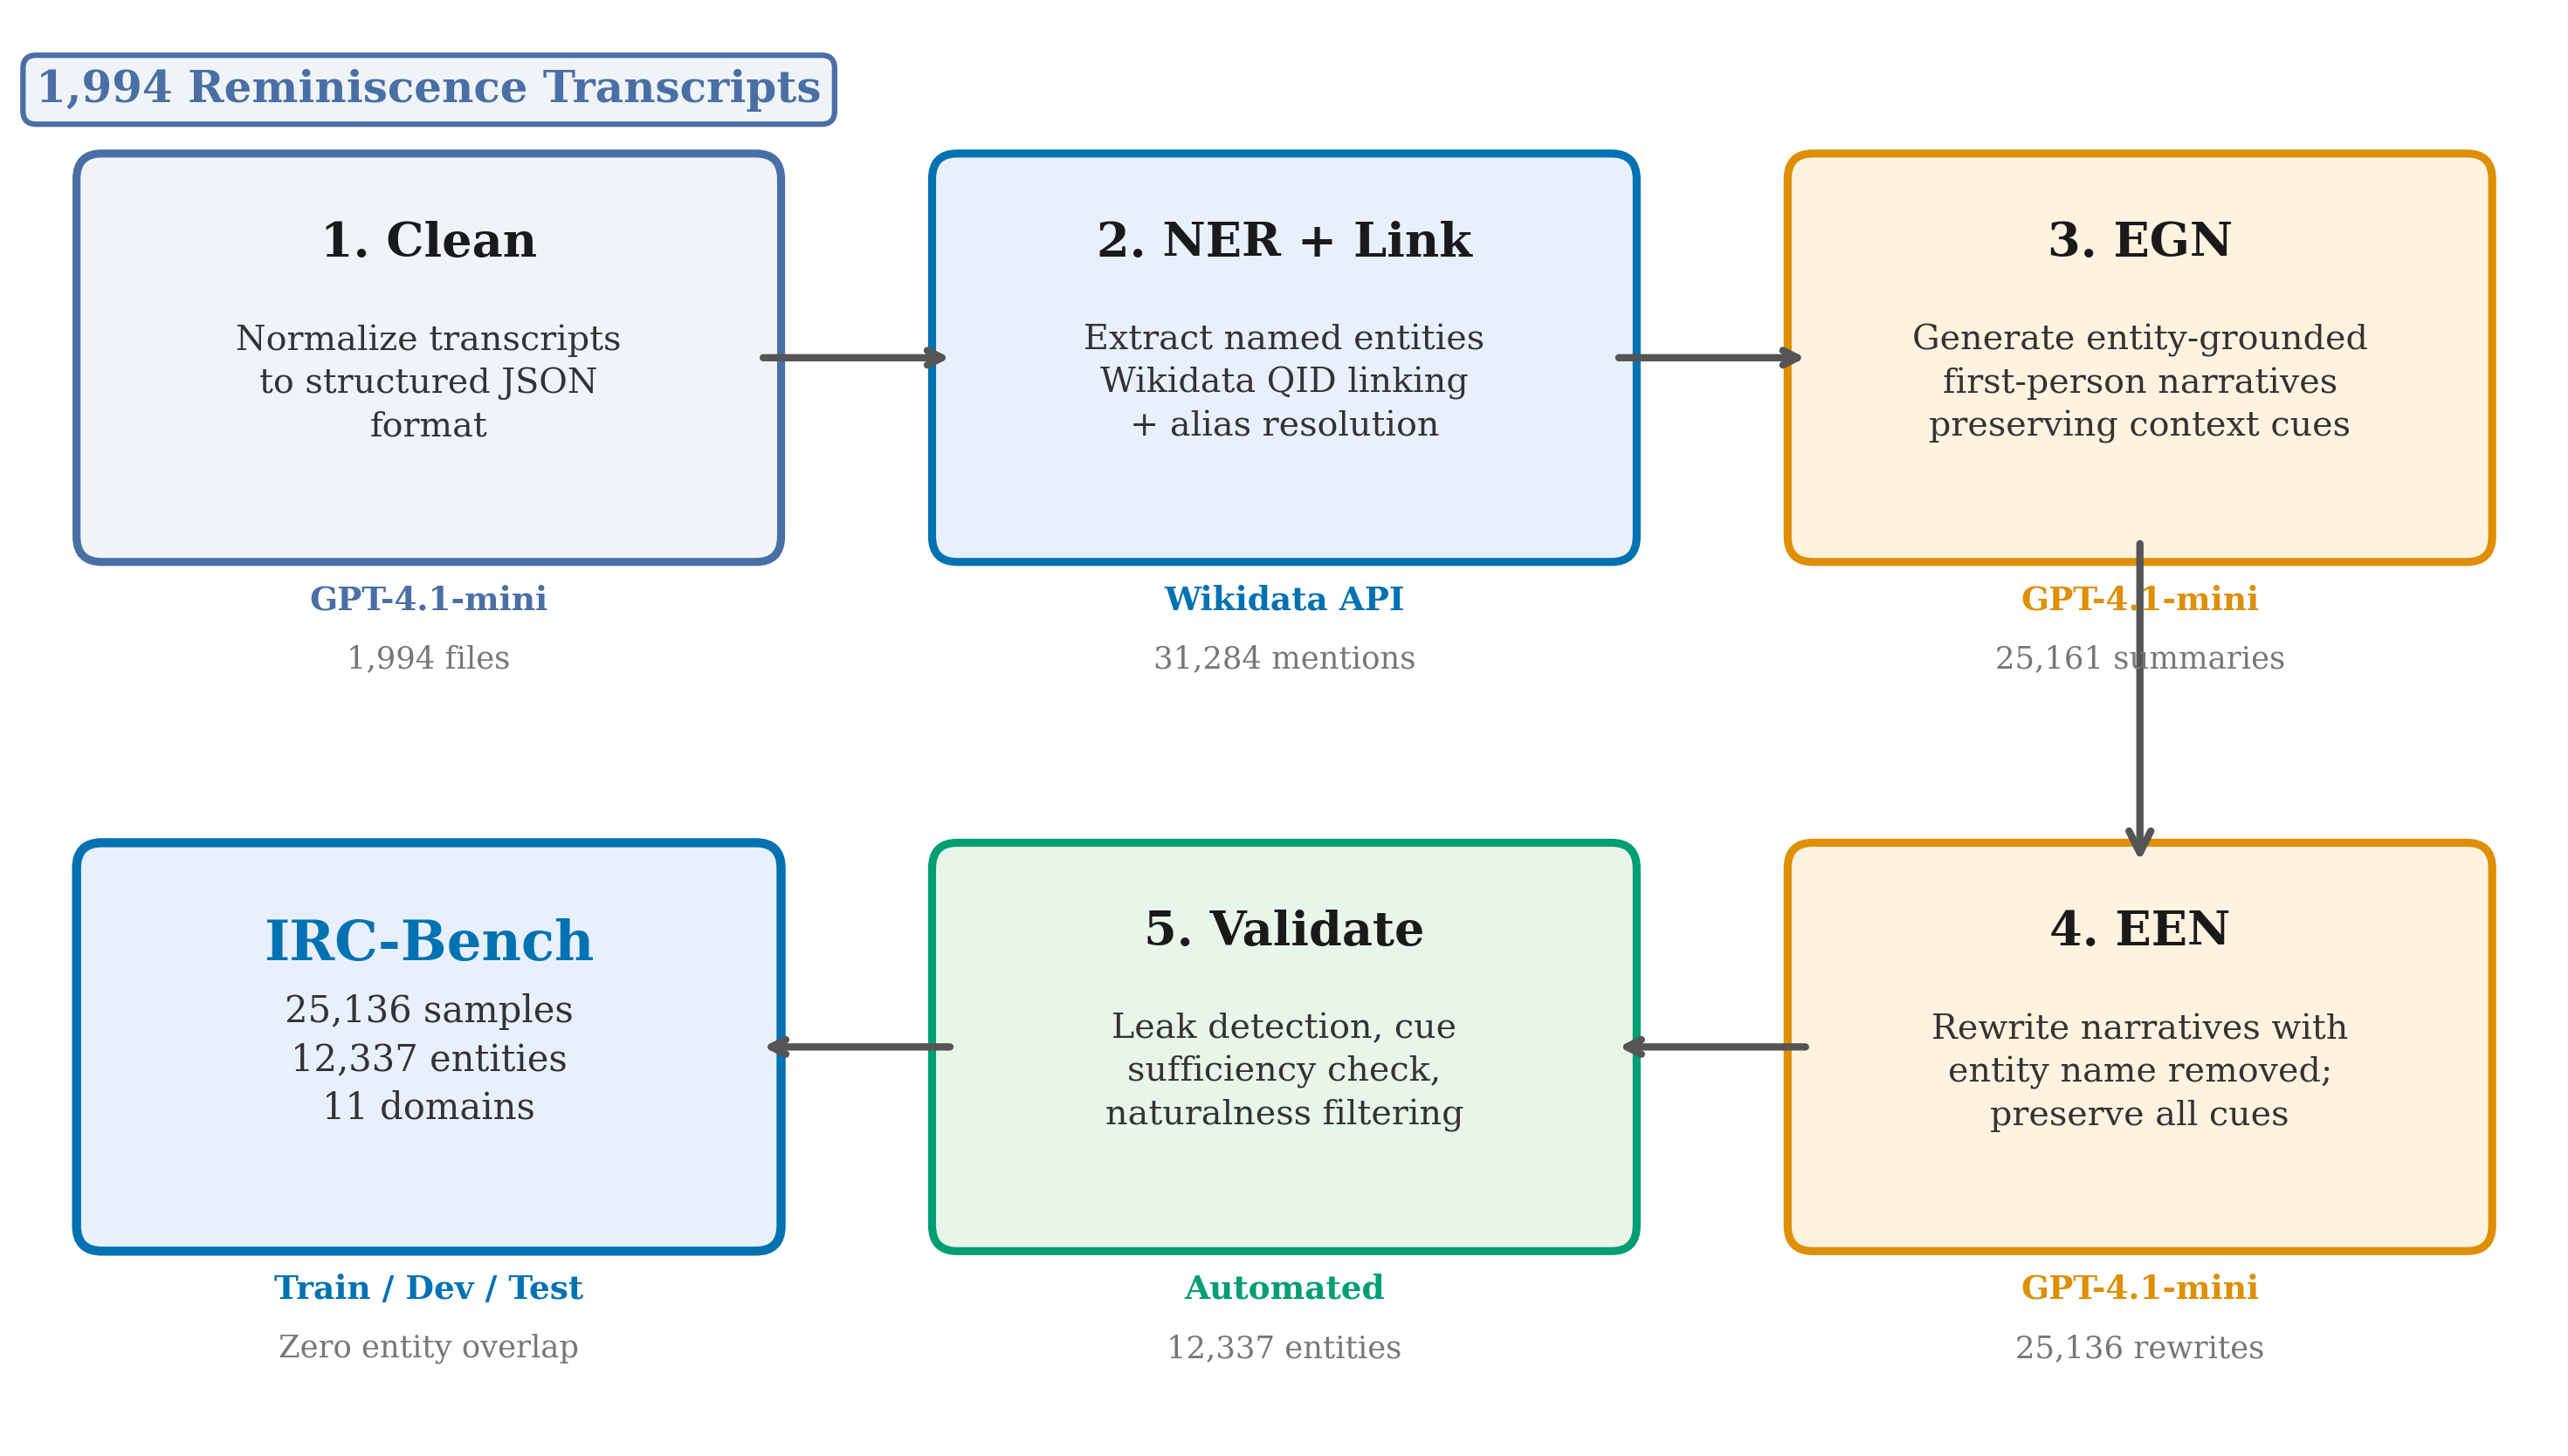
\includegraphics[width=5.83333in,height=3.3084in,alt={IRC-Bench construction pipeline}]{pandoc-media/media/image1.png}

\textbf{Figure 1:} IRC-Bench construction pipeline. Raw oral history
transcripts undergo cleaning, NER with Wikidata linking, entity-grounded
narrative generation, and entity elision to produce implicit entity
recognition samples.

\subsection{4 ~ Methodology}\label{methodology}

\subsubsection{4.1 ~ Task Formulation}\label{task-formulation}

Given a first-person narrative text \(t\) that implicitly references a
named entity \(e\) without ever mentioning \(e\) by name, the task is to
identify \(e\). We evaluate under two formulations. In the
\textbf{open-world} setting, the model generates the entity name as
free-form text without access to a candidate set. In the
\textbf{closed-world} setting, the model ranks all 12,337 entities in
the knowledge base by relevance to the query.

\subsubsection{4.2 ~ The Non-Locality
Property}\label{the-non-locality-property}

We define a key structural property distinguishing implicit entity
recognition from span-based tasks. Let
\(C\left( T,e^{*} \right) = \{ c_{1},c_{2},\ldots,c_{n}\}\) denote the
set of textual cues in \(T\) that collectively identify \(e^{*}\). In
NER and EL, the entity is localized in a contiguous span. In implicit
entity recognition, the entity is \emph{non-local}:

\[exists\, m \subset T\mspace{6mu} exts.t.\mspace{6mu} m\mspace{6mu} extiscontiguous \land m \Rightarrow e^{*}\]

\[extbut\mspace{6mu} C\left( T,e^{*} \right) \Rightarrow e^{*},\mspace{6mu} c_{i}\mspace{6mu} extnon - contiguous\]

No single contiguous substring suffices, but the distributed cues
collectively determine the entity. We validate this empirically: GPT-4o
zero-shot accuracy on full implicit texts reaches 33.5\%, while
single-sentence accuracy drops to 12.9\% (n=200), confirming that
recognition requires integrating cues distributed across the entire
passage.

\subsubsection{4.3 ~ Open-World Methods}\label{open-world-methods}

We evaluate LLMs in a generative setting with zero-shot (ZS), few-shot
(FS, 5 demonstrations), and chain-of-thought (CoT) prompting. Models
include GPT-4o {[}20{]}, GPT-4.1-mini, and Llama 3.1 8B Instruct
{[}21{]}. Direct prompting uses temperature 0.0; CoT uses temperature
0.7 with 300 output tokens. We additionally fine-tune Llama 3.1 8B using
QLoRA {[}22, 23{]} with 4-bit NF4 quantization, LoRA rank 16, alpha 32,
and 2 epochs on the train split. The entity-level split guarantees the
model cannot memorize entity-specific patterns.

\subsubsection{4.4 ~ Closed-World Methods}\label{closed-world-methods}

We encode both implicit query text and entity representations into a
shared embedding space, ranking by cosine similarity. We explore three
entity representations: \emph{Name} (entity name alone),
\emph{Description} (name + LLM-generated description), and \emph{Wiki}
(first Wikipedia sentence). We evaluate BAAI/bge-base-en-v1.5 {[}24{]}
off-the-shelf and fine-tuned via Dense Passage Retrieval (DPR) {[}25{]}
with Multiple Negatives Ranking Loss (3 epochs, batch size 48, learning
rate 2e-5).

\subsubsection{4.5 ~ RAG Baseline}\label{rag-baseline}

A hybrid pipeline retrieves top-5 candidates via BGE-base, then
GPT-4.1-mini reranks and selects the most likely entity. This tests
whether LLM reranking can improve over pure embedding retrieval.

\subsubsection{4.6 ~ Evaluation Protocol}\label{evaluation-protocol}

We employ a four-tier matching hierarchy: (1) exact string match, (2)
alias match via Wikidata, (3) containment match (substring), and (4)
Jaccard similarity ≥ 0.5. The primary open-world metric is alias-aware
accuracy (Tiers 1+2). Closed-world experiments report Hit@K, MRR, and
alias-aware Hit@1. All key comparisons use McNemar\textquotesingle s
test for significance.

\subsection{5 ~ Results}\label{results}

\subsubsection{5.1 ~ Open-World
Performance}\label{open-world-performance}

Table 3 presents the open-world results. QLoRA-adapted Llama 3.1 8B
(O10) achieves the highest exact match at 38.94\%, substantially
outperforming all non-fine-tuned methods. Among direct prompting, GPT-4o
few-shot (O2) is strongest at 31.62\% exact match. Model scale is the
dominant zero-shot factor: Llama 3.1 8B (13.92\%) to GPT-4.1-mini
(25.71\%) to GPT-4o (27.02\%). Few-shot prompting consistently improves
all models (p \textless{} 0.001).

QLoRA fine-tuning nearly triples the base Llama\textquotesingle s
zero-shot performance (13.92\% to 38.94\%) and exceeds GPT-4o few-shot
by 7.32 pp, despite the entity-level split ensuring zero overlap with
training entities. At the Jaccard level, O10 reaches 51.59\%, meaning
more than half of predictions are at least partially correct.

Chain-of-thought prompting degrades all models: GPT-4o drops from
33.30\% (ZS alias) to 23.89\%, GPT-4.1-mini from 25.71\% (ZS exact) to
18.93\%, and Llama 3.1 8B from 13.92\% to 6.22\%. Temperature control
experiments confirm CoT structurally harms smaller models, while for
GPT-4o, controlling temperature recovers parity with zero-shot but does
not exceed it. The RAG approach (19.71\% exact) underperforms even
GPT-4.1-mini zero-shot (25.71\%).

\textbf{Table 3:} Open-world results on IRC-Bench test set (n=4,633).
Best in each column is highlighted.

{\def\LTcaptype{none} % do not increment counter
\begin{longtable}[]{@{}
  >{\raggedright\arraybackslash}p{(\linewidth - 12\tabcolsep) * \real{0.0849}}
  >{\raggedright\arraybackslash}p{(\linewidth - 12\tabcolsep) * \real{0.2442}}
  >{\raggedright\arraybackslash}p{(\linewidth - 12\tabcolsep) * \real{0.1348}}
  >{\raggedright\arraybackslash}p{(\linewidth - 12\tabcolsep) * \real{0.1239}}
  >{\raggedright\arraybackslash}p{(\linewidth - 12\tabcolsep) * \real{0.1188}}
  >{\raggedright\arraybackslash}p{(\linewidth - 12\tabcolsep) * \real{0.1489}}
  >{\raggedright\arraybackslash}p{(\linewidth - 12\tabcolsep) * \real{0.1443}}@{}}
\toprule\noalign{}
\begin{minipage}[b]{\linewidth}\raggedright
ID
\end{minipage} & \begin{minipage}[b]{\linewidth}\raggedright
Model
\end{minipage} & \begin{minipage}[b]{\linewidth}\raggedright
Mode
\end{minipage} & \begin{minipage}[b]{\linewidth}\raggedright
Exact (\%)
\end{minipage} & \begin{minipage}[b]{\linewidth}\raggedright
Alias (\%)
\end{minipage} & \begin{minipage}[b]{\linewidth}\raggedright
Contain (\%)
\end{minipage} & \begin{minipage}[b]{\linewidth}\raggedright
Jaccard (\%)
\end{minipage} \\
\midrule\noalign{}
\endhead
\bottomrule\noalign{}
\endlastfoot
O1 & GPT-4o & Zero-shot & 27.02 & 33.30 & 33.30 & 35.05 \\
O2 & GPT-4o & Few-shot & 31.62 & 38.94 & 38.94 & 41.10 \\
O3 & GPT-4.1-mini & Zero-shot & 25.71 & 27.09 & 33.50 & 35.94 \\
O4 & GPT-4.1-mini & Few-shot & 28.66 & 36.89 & 36.89 & 39.48 \\
O5 & Llama 3.1 8B & Zero-shot & 13.92 & 14.81 & 19.47 & 20.18 \\
O6 & Llama 3.1 8B & Few-shot & 17.83 & 18.80 & 24.61 & 25.66 \\
O10 & Llama 3.1 8B (QLoRA) & Fine-tuned & 38.94 & 41.42 & 47.90 &
51.59 \\
O11 & GPT-4.1-mini CoT & t=0.7 & 18.93 & 20.27 & 26.48 & 27.69 \\
O12 & GPT-4o CoT & t=0.7 & 22.51 & 23.89 & 30.91 & 32.33 \\
O13 & Llama 3.1 8B CoT & t=0.7 & 6.22 & 6.69 & 11.72 & 12.24 \\
RAG1 & BGE + GPT-4.1-mini & RAG & 19.71 & 20.53 & 28.75 & 29.55 \\
\end{longtable}
}

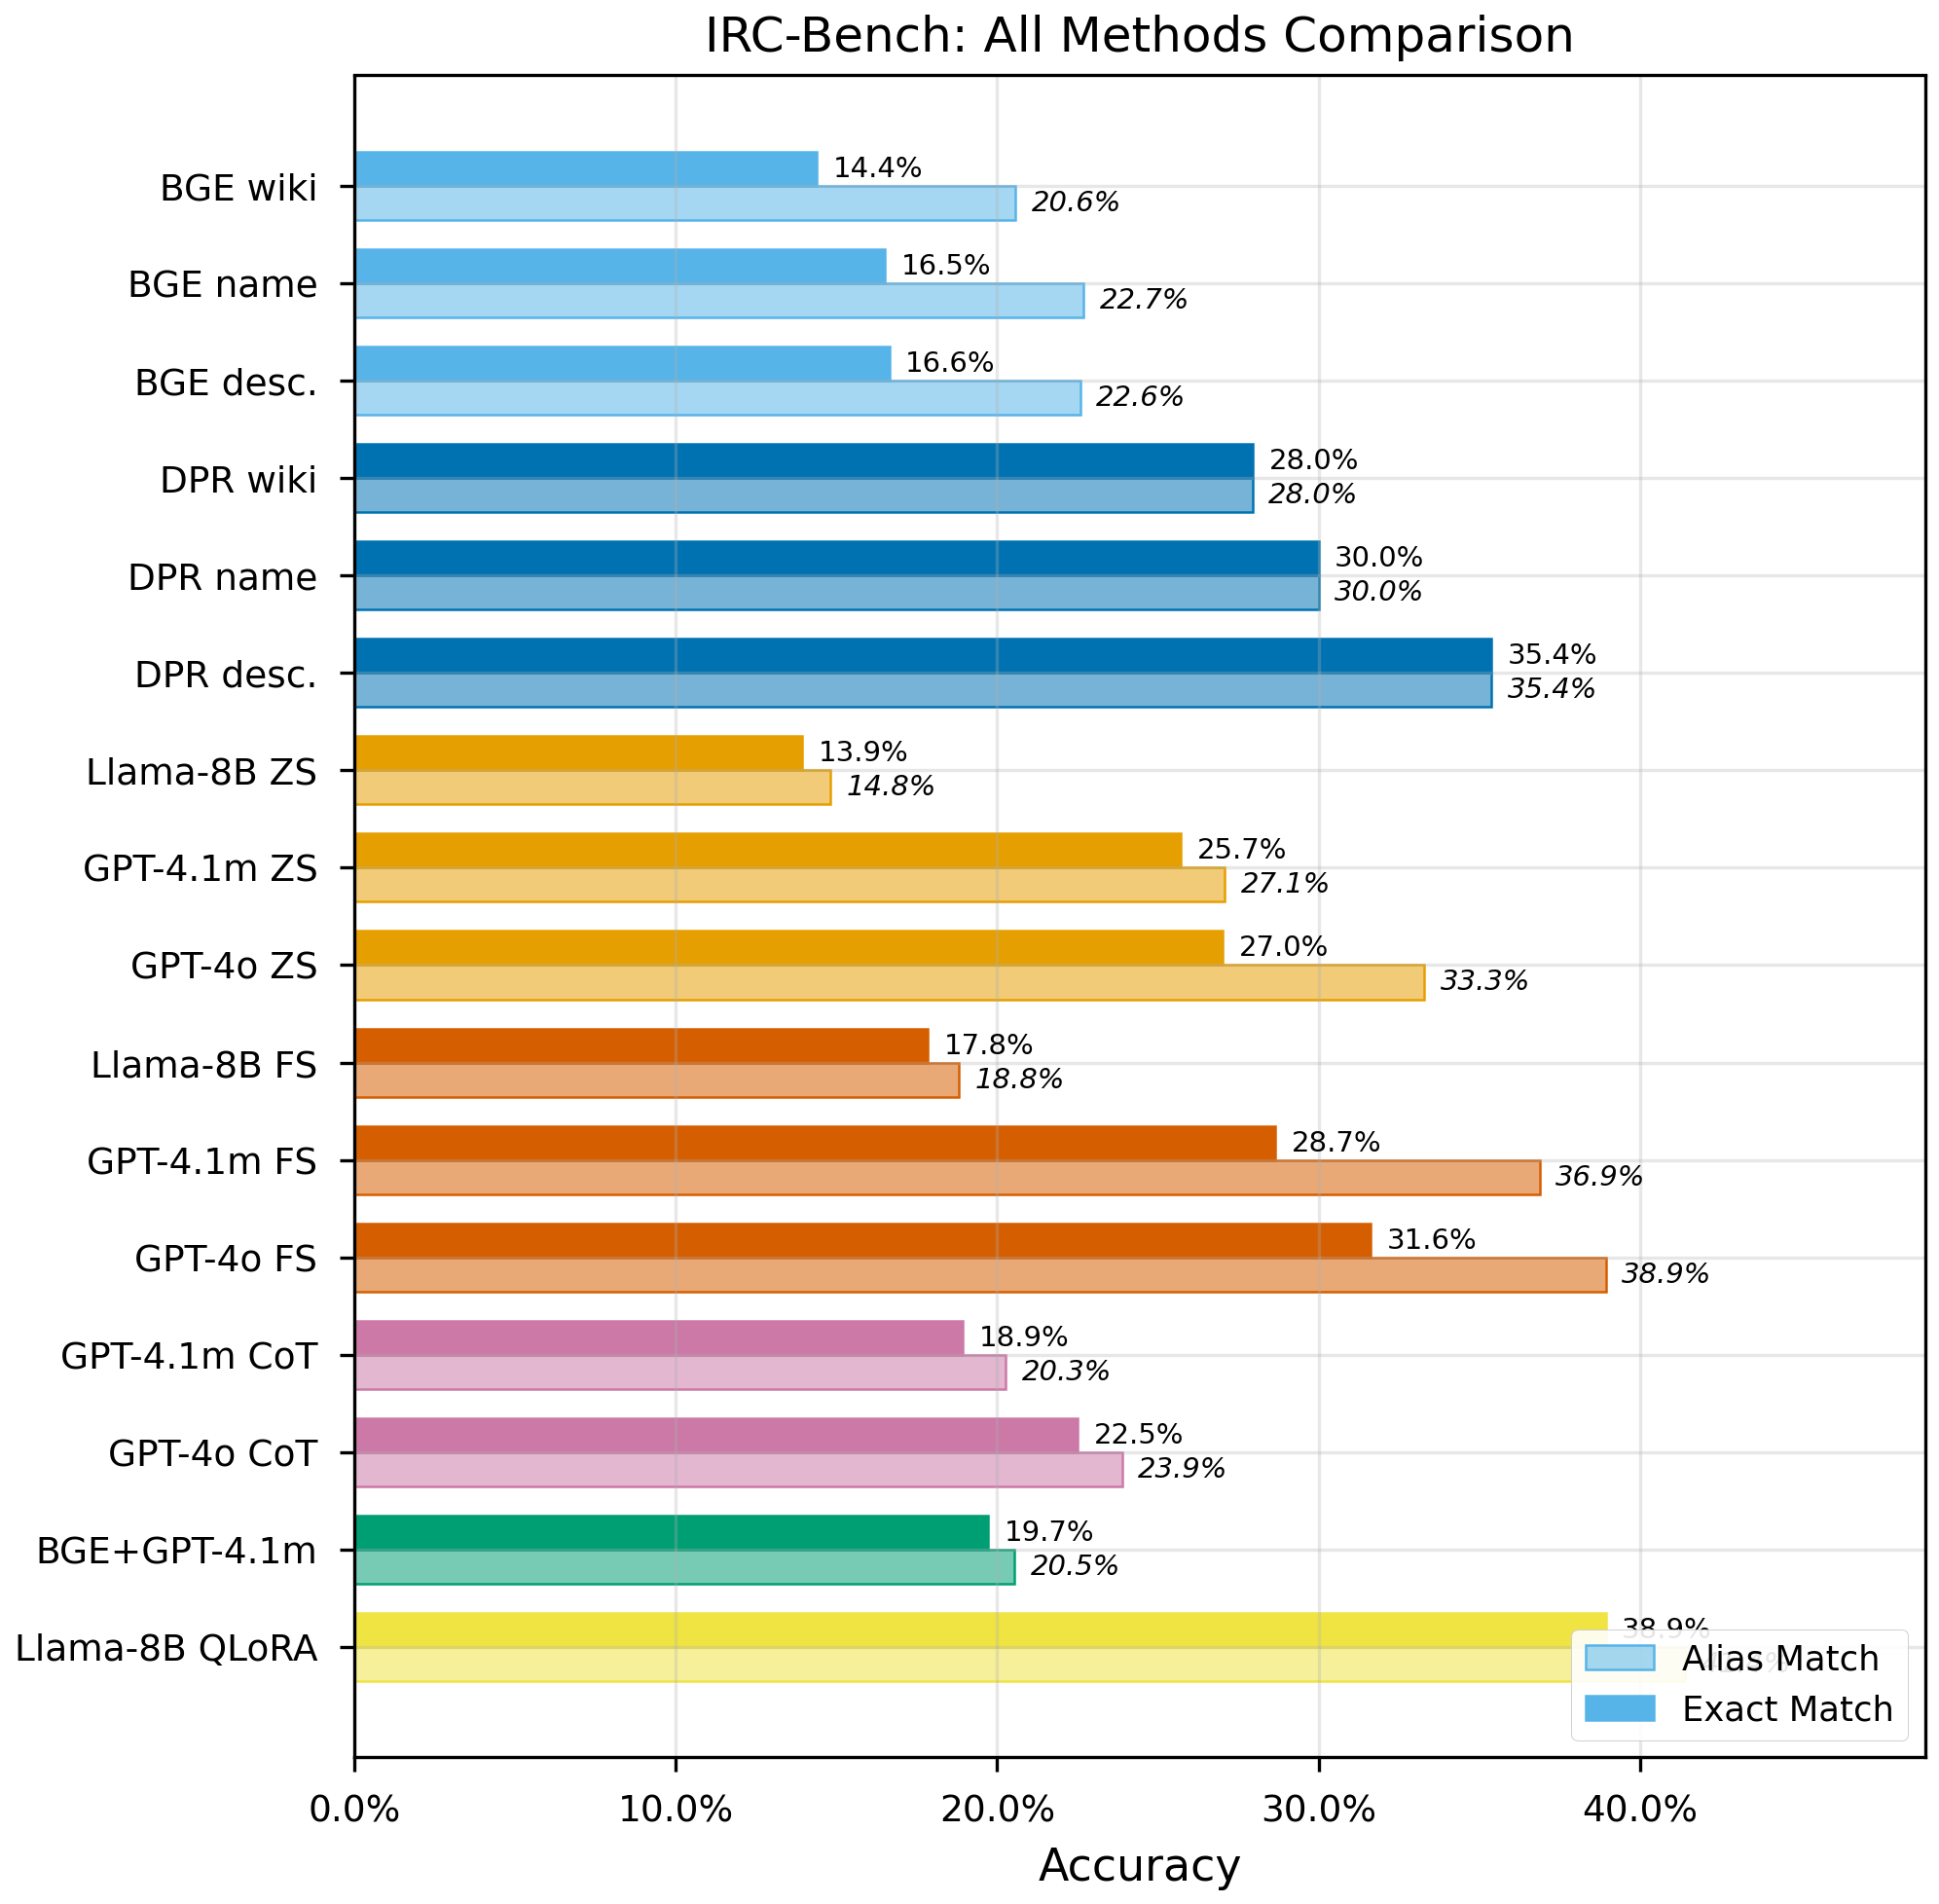
\includegraphics[width=5.83333in,height=5.72791in,alt={Main results comparison across all methods}]{pandoc-media/media/image2.png}

\textbf{Figure 2:} Comparison of open-world and closed-world methods on
IRC-Bench. Open-world methods measured by exact match and alias-aware
accuracy; closed-world methods by Hit@1 and Hit@10.

\subsubsection{5.2 ~ Closed-World
Performance}\label{closed-world-performance}

Table 4 shows closed-world retrieval results. Fine-tuned DPR with
descriptions (C5) achieves 35.38\% Hit@1, 71.49\% Hit@10, and 0.4751
MRR. With alias-aware evaluation, C5 reaches 42.80\% Hit@1. DPR
fine-tuning more than doubles Hit@1 for all entity representations: Name
(16.51\% to 30.00\%), Description (16.64\% to 35.38\%), Wiki (14.38\% to
27.95\%). The largest absolute gain occurs for descriptions (+18.74 pp),
indicating that fine-tuning is especially effective at aligning
narrative cue structure with rich attribute content. Entity descriptions
consistently outperform name-only and Wikipedia representations across
both retrieval architectures.

\textbf{Table 4:} Closed-world retrieval results. Candidate set: 12,337
entities. Best in each column is highlighted.

{\def\LTcaptype{none} % do not increment counter
\begin{longtable}[]{@{}
  >{\raggedright\arraybackslash}p{(\linewidth - 16\tabcolsep) * \real{0.0517}}
  >{\raggedright\arraybackslash}p{(\linewidth - 16\tabcolsep) * \real{0.1517}}
  >{\raggedright\arraybackslash}p{(\linewidth - 16\tabcolsep) * \real{0.1514}}
  >{\raggedright\arraybackslash}p{(\linewidth - 16\tabcolsep) * \real{0.1054}}
  >{\raggedright\arraybackslash}p{(\linewidth - 16\tabcolsep) * \real{0.1054}}
  >{\raggedright\arraybackslash}p{(\linewidth - 16\tabcolsep) * \real{0.1054}}
  >{\raggedright\arraybackslash}p{(\linewidth - 16\tabcolsep) * \real{0.1196}}
  >{\raggedright\arraybackslash}p{(\linewidth - 16\tabcolsep) * \real{0.0994}}
  >{\raggedright\arraybackslash}p{(\linewidth - 16\tabcolsep) * \real{0.1099}}@{}}
\toprule\noalign{}
\begin{minipage}[b]{\linewidth}\raggedright
ID
\end{minipage} & \begin{minipage}[b]{\linewidth}\raggedright
Retriever
\end{minipage} & \begin{minipage}[b]{\linewidth}\raggedright
Entity Repr.
\end{minipage} & \begin{minipage}[b]{\linewidth}\raggedright
Hit@1 (\%)
\end{minipage} & \begin{minipage}[b]{\linewidth}\raggedright
Hit@3 (\%)
\end{minipage} & \begin{minipage}[b]{\linewidth}\raggedright
Hit@5 (\%)
\end{minipage} & \begin{minipage}[b]{\linewidth}\raggedright
Hit@10 (\%)
\end{minipage} & \begin{minipage}[b]{\linewidth}\raggedright
MRR
\end{minipage} & \begin{minipage}[b]{\linewidth}\raggedright
Alias H@1 (\%)
\end{minipage} \\
\midrule\noalign{}
\endhead
\bottomrule\noalign{}
\endlastfoot
C1 & BGE (off-the-shelf) & Name & 16.51 & 26.38 & 30.97 & 36.76 & 0.2362
& 22.08 \\
C2 & BGE (off-the-shelf) & Description & 16.64 & 27.78 & 33.41 & 40.60 &
0.2480 & 21.78 \\
C3 & BGE (off-the-shelf) & Wiki & 14.38 & 25.10 & 29.92 & 37.32 & 0.2211
& 19.32 \\
C4 & DPR (fine-tuned) & Name & 30.00 & 46.36 & 53.66 & 63.31 & 0.4131 &
37.10 \\
C5 & DPR (fine-tuned) & Description & 35.38 & 53.51 & 61.82 & 71.49 &
0.4751 & 42.80 \\
C6 & DPR (fine-tuned) & Wiki & 27.95 & 44.98 & 51.82 & 59.55 & 0.3851 &
34.38 \\
\end{longtable}
}

\subsubsection{5.3 ~ Key Findings}\label{key-findings}

\textbf{Finding 1: Fine-tuning is the most impactful intervention.}
QLoRA raises exact match from 13.92\% to 38.94\% (2.80x). DPR
fine-tuning raises Hit@1 from 16.64\% to 35.38\% (2.13x). Both achieve
these gains despite zero entity overlap between train and test sets.

\textbf{Finding 2: Chain-of-thought degrades all models.} CoT reduces
GPT-4o from 33.30\% to 23.89\% (alias), GPT-4.1-mini from 25.71\% to
18.93\% (exact), and Llama 8B from 13.92\% to 6.22\%. Temperature
control experiments confirm this is structural for smaller models; for
GPT-4o, controlling temperature recovers parity with zero-shot but does
not exceed it.

\textbf{Finding 3: RAG underperforms direct LLM inference.} RAG1
(19.71\%) is 8.95 pp below GPT-4.1-mini few-shot (28.66\%). The
retrieval bottleneck (gold entity in top-5 only 33\% of the time) is the
limiting factor.

\textbf{Finding 4: Model scale dominates zero-shot performance.} GPT-4o
ZS (27.02\%) outperforms Llama 8B ZS (13.92\%) by 13.10 pp (p
\textless{} 0.001). The retriever\textquotesingle s Hit@10 of 71.49\%
reveals strong latent signal for future DPR+LLM reranking approaches.

\textbf{Finding 5: Entity descriptions are the best retrieval
representation.} C5 (DPR+Desc) outperforms C4 (DPR+Name) by 5.38 pp on
Hit@1 and C6 (DPR+Wiki) by 7.43 pp. The pattern holds for off-the-shelf
BGE as well.

\subsection{6 ~ Discussion}\label{discussion}

The failure of chain-of-thought prompting is the most counterintuitive
finding. CoT improves mathematical reasoning and multi-hop QA by
decomposing complex problems {[}26{]}, yet it degrades implicit entity
recognition. The explanation lies in the gestalt nature of the task:
identifying an implicit entity requires simultaneously attending to a
constellation of distributed cues and matching this constellation
against parametric knowledge. When forced to reason step by step, models
fixate on individual cues in isolation, arriving at locally plausible
but globally incorrect entities. Temperature control experiments confirm
CoT is structurally harmful for smaller models (GPT-4.1-mini: +0.5pp at
t=0.0, still 6.3pp below ZS), while for GPT-4o, controlling temperature
recovers the gap to ZS parity without exceeding it.

The RAG pipeline underperforms direct generation because dense
retrievers encode the EEN as a single vector, losing fine-grained cue
information. Retrieved candidates are topically related but often
incorrect, and when presented as context they can override the
model\textquotesingle s own correct intuition. With BGE-base, the gold
entity appears in the top-5 only 33.41\% of the time, severely limiting
the reranker.

The success of QLoRA despite zero entity overlap indicates that
fine-tuning teaches transferable skills: the task format (extracting a
single canonical name), cue integration patterns (which temporal,
spatial, and relational combinations are diagnostic), and entity type
priors (calibrating expectations to reduce wrong-type errors). The model
learns "how to solve implicit entity puzzles" rather than memorizing
specific answers. Comparing the best open-world (O10: 38.94\%) and
closed-world (C5: 35.38\% Hit@1, 42.80\% alias) results, both paradigms
reach roughly comparable alias-level performance, though the
closed-world Hit@10 of 71.49\% suggests that combining fine-tuned
retrieval shortlists with fine-tuned LLM reranking is a promising future
direction.

Benchmark calibration validates the dataset\textquotesingle s
difficulty: an automated quality assessment (n=500, GPT-4o judge) found
42\% of samples recoverable by informed judgment, closely matching the
best system\textquotesingle s alias accuracy (41.4\%), suggesting top
models approach the practical ceiling imposed by available cues. EEN
naturalness averaged 4.87/5. Limitations include the English-only,
American-focused scope; LLM-generated entity elision (though validated);
alias-aware evaluation that still penalizes unregistered surface forms;
and QLoRA\textquotesingle s max\_seq=192 tokens truncating approximately
6\% of prompts.

\subsection{7 ~ Conclusion}\label{conclusion}

We have extended implicit entity recognition to long-form reminiscence
narratives, formalizing the non-locality property and releasing
IRC-Bench with 25,136 samples from 12,337 Wikidata-linked entities
across 1,994 oral history transcripts. Our evaluation of 19
configurations reveals that fine-tuning is the most impactful
intervention (QLoRA achieving 38.94\% exact match, nearly tripling the
base model), chain-of-thought prompting consistently degrades
performance, and RAG underperforms direct inference due to the
non-locality of implicit cues. Future work should explore combining DPR
shortlists with LLM reranking (leveraging C5\textquotesingle s 71.49\%
Hit@10), cross-lingual benchmarks, and architectures that explicitly
model distributed cue structure.

\subsection{References}\label{references}

{[}1{]} Subramaniam, P. and Woods, B. (2012). The impact of individual
reminiscence therapy for people with dementia. \emph{Expert Review of
Neurotherapeutics}, 12(5):545-555.

{[}2{]} Boyd, D. A. (2012). Achieving the promise of oral history in a
digital age. In Ritchie, D. A., editor, \emph{The Oxford Handbook of
Oral History}. Oxford University Press.

{[}3{]} Nadeau, D. and Sekine, S. (2007). A survey of named entity
recognition and classification. \emph{Lingvisticae Investigationes},
30(1):3-26.

{[}4{]} Li, J., Sun, A., Han, J., and Li, C. (2022). A survey on deep
learning for named entity recognition. \emph{IEEE TKDE}, 34(1):50-70.

{[}5{]} Ganea, O.-E. and Hofmann, T. (2017). Deep joint entity
disambiguation with local neural attention. In \emph{Proc. EMNLP}, pages
2619-2629.

{[}6{]} Kolitsas, N., Ganea, O.-E., and Hofmann, T. (2018). End-to-end
neural entity linking. In \emph{Proc. CoNLL}, pages 519-529.

{[}7{]} Lee, K., He, L., Lewis, M., and Zettlemoyer, L. (2017).
End-to-end neural coreference resolution. In \emph{Proc. EMNLP}, pages
188-197.

{[}8{]} Hosseini, H. (2022). Implicit entity recognition and linking in
tweets. PhD thesis, Toronto Metropolitan University.

{[}9{]} Hosseini, H. and Bagheri, E. (2021). Learning to rank implicit
entities on Twitter. \emph{Information Processing \& Management},
58(3):102503.

{[}10{]} Perera, N., Dehmer, M., and Emmert-Streib, F. (2020). Named
entity recognition and relation detection for biomedical information
extraction. \emph{Frontiers in Cell and Dev. Biology}, 8:673.

{[}11{]} Hou, Y. (2020). Bridging anaphora resolution as question
answering. In \emph{Proc. ACL}, pages 1428-1438.

{[}12{]} Poesio, M., Stuckardt, R., and Versley, Y. (2016).
\emph{Anaphora Resolution: Algorithms, Resources, and Applications}.
Springer.

{[}13{]} Nikitina, S., Callaioli, S., and Baez, M. (2018). Smart
conversational agents for reminiscence. \emph{Proc. 1st Intl. Workshop
on Software Engineering for Cognitive Services}, 52-57.

{[}14{]} Lazar, A., Demiris, G., and Thompson, H. (2016). Evaluation of
a multifunctional technology system in a memory care unit.
\emph{Informatics for Health and Social Care}, 41(4):373-389.

{[}15{]} Lample, G., Ballesteros, M., Subramanian, S., Kawakami, K., and
Dyer, C. (2016). Neural architectures for named entity recognition. In
\emph{Proc. NAACL}, pages 260-270.

{[}16{]} Pessanha, F. and Akdag Salah, A. (2022). A computational look
at oral history archives. \emph{ACM JOCCH}, 15(1):6:1-6:16.

{[}17{]} Yang, Z., Qi, P., Zhang, S., et al. (2018). HotpotQA: A dataset
for diverse, explainable multi-hop question answering. In \emph{Proc.
EMNLP}.

{[}18{]} Petroni, F., Rocktaschel, T., Riedel, S., et al. (2019).
Language models as knowledge bases? In \emph{Proc. EMNLP}.

{[}19{]} Lewis, P., Perez, E., Piktus, A., et al. (2020).
Retrieval-augmented generation for knowledge-intensive NLP tasks. In
\emph{Proc. NeurIPS}.

{[}20{]} OpenAI (2024). GPT-4o system card. \emph{Technical Report}.

{[}21{]} Dubey, A., et al. (2024). The Llama 3 herd of models.
\emph{arXiv:2407.21783}.

{[}22{]} Hu, E. J., Shen, Y., Wallis, P., et al. (2022). LoRA: Low-rank
adaptation of large language models. In \emph{Proc. ICLR}.

{[}23{]} Dettmers, T., Pagnoni, A., Holtzman, A., and Zettlemoyer, L.
(2023). QLoRA: Efficient finetuning of quantized language models. In
\emph{Proc. NeurIPS}.

{[}24{]} Xiao, S., Liu, Z., Zhang, P., et al. (2023). C-Pack: Packaged
resources to advance general Chinese embedding. \emph{arXiv:2309.07597}.

{[}25{]} Karpukhin, V., Oguz, B., Min, S., et al. (2020). Dense passage
retrieval for open-domain question answering. In \emph{Proc. EMNLP},
pages 6769-6781.

{[}26{]} Wei, J., Wang, X., Schuurmans, D., et al. (2022).
Chain-of-thought prompting elicits reasoning in large language models.
In \emph{Proc. NeurIPS}.

{[}27{]} Butler, R. N. (1963). The life review: An interpretation of
reminiscence in the aged. \emph{Psychiatry}, 26(1), 65-76.

{[}28{]} Wu, L., Petroni, F., Josifoski, M., Riedel, S., and
Zettlemoyer, L. (2020). Scalable zero-shot entity linking with dense
entity retrieval. In \emph{Proc. EMNLP}, pages 6397-6407.

{[}29{]} Devlin, J., Chang, M.-W., Lee, K., and Toutanova, K. (2019).
BERT: Pre-training of deep bidirectional transformers for language
understanding. In \emph{Proc. NAACL}, pages 4171-4186.

{[}30{]} De Cao, N., Izacard, G., Riedel, S., and Petroni, F. (2021).
Autoregressive entity retrieval. In \emph{Proc. ICLR}.

The NeurIPS Paper Checklist is provided as a separate document.

\end{document}
